\begin{partbacktext}
\part{Safety Solutions}\label{chap:verification}
%\noindent Use the template \emph{part.tex} together with the document class SVMono (monograph-type books) or SVMult (edited books) to style your part title page and, if desired, a short introductory text (maximum one page) on its verso page.

After discovering safety vulnerabilities through algorithms in the previous part, it is a natural next step to consider safety solutions. In this part, we consider two major approaches:  verification and enhancement. The relation between attack, verification, and enhancement is given in Figure~\ref{fig:safetyFramework}. Once safety attacks identify safety vulnerabilities of certain safety properties, the dedicated enhancement will be applied to improve the machine learning models before passing over to the safety verification, which in turn determines whether the safety properties hold. Once an affirmative answer is reported, we conclude that the enhanced model is safe with respect to the property. Otherwise, we will repeat the above process.   

\begin{figure}[!htbp]
    \centering
    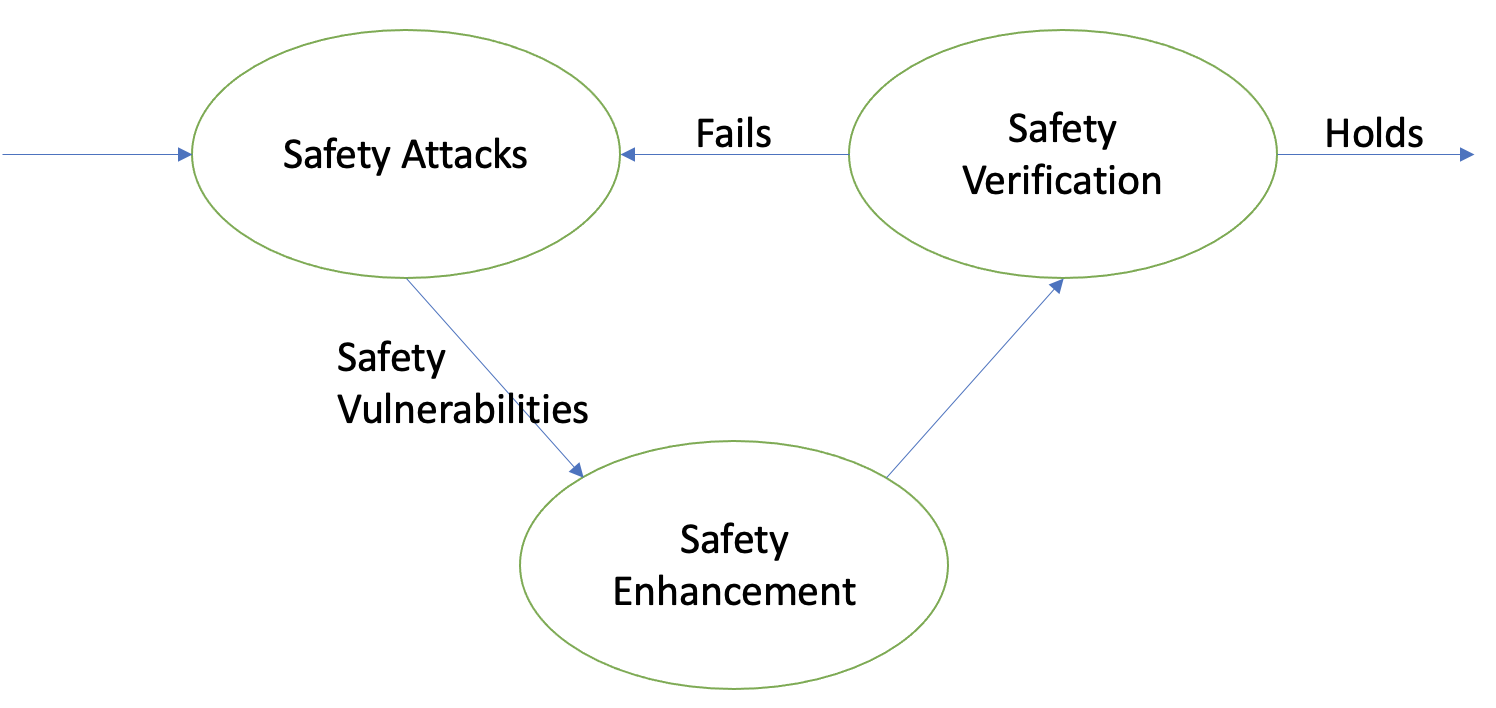
\includegraphics[width=0.8\textwidth]{images/robustnessVerification/framework.png}
    \caption{Interactions of Safety Attacks (Part \ref{part:simple}) with two Safety Solutions to be discussed in this Part}
    \label{fig:safetyFramework}
\end{figure}


%This chapter considers the formal verification techniques on deep neural networks. 
Verification is a collection of techniques that, given a model (e.g., a trained machine learning model) and a property, automatically determine whether a property holds on the model. Unlike safety attacks, the verification algorithm can conclude the existence or non-existence of safety vulnerabilities with mathematical proof. Therefore, it contributes as a key step in software development to ensure that the software achieves its design specification/requirement. 
%
Currently, verification for machine learning is still in its infancy, and we will focus on a recent surge in the verification of robustness property over the feedforward neural network. 

Enhancement is usually specific with respect to the property under consideration. We discuss two typical enhancements in Chapter~\ref{chap:advtraining}, for robustness and privacy, respectively. Robustness enhancement is conducted through adversarial training, which considers adversarial examples during the training process. On the other hand, privacy enhancement is conducted through randomisation, by adding noises to either the training or the inference. 

\end{partbacktext}